\documentclass[11pt]{article}
\usepackage{fullpage, amsmath, graphicx, float}
\usepackage[linesnumbered,ruled,vlined]{algorithm2e}
\usepackage{amsthm}
\renewcommand{\baselinestretch}{1.02}
\newcommand{\Q}[1]{\medskip\item {[{\em #1 marks\/}]}\ }
\usepackage{xcolor}
%\newif\ifsol
%\solfalse
%\newcommand{\solution}[1]{{\ifsol \color{red} {#1} \fi}}

\newtheorem{claim}{Claim}

\newcommand{\down}[1]{\left\lfloor #1\right\rfloor}
\newcommand{\up}[1]{\left\lceil #1\right\rceil}

\begin{document}
%\thispagestyle{empty}

\hfill CS 341, Spring 2020\par
\hfill Semih Salihoglu

\bigskip
\begin{center}\large\bf Assignment 2 (due Sunday, June 21, midnight EST)
\end{center}

\noindent{\bf Instructions:}
\begin{itemize}
\item Hand in your assignment using Crowdmark. Detailed instructions are on the course website.
\item Give complete legible solutions to all questions.
\item Your answers will be marked for clarity as well as correctness.
\item For any algorithm you present, you should justify its correctness
(if it is not obvious) and analyze the complexity.
\end{itemize}

\begin{enumerate}

\Q{12} Consider the following recurrence:

$$T(n) = \left\{\begin{array}{ll}
T(\lfloor n/4 \rfloor) + T(\lfloor n/9 \rfloor) + T(\lfloor n/36 \rfloor) + 2016 & \text{ if }  n \geq 36\\
341 & \text{ if }1 \le n \le 35.
\end{array}\right.$$

Prove inductively (i.e., with the guess-and-check or substitution method) the upper bound $T(n) = O(\sqrt{n})$.
[Hint: use $T(n) \le c\sqrt{n} - c'$ as the ``guess'', where $c$ and $c'$ are suitable constants.]

We calim that $T(n) \leq 1349 \sqrt{n} - 1008$.\\
\textbf{Base Case:} $1 \leq n \leq 35$. 

\begin{align*}
    T(n) & = 341 \\
    & \leq 1349 - 1008 \\
    & \leq 1349 \sqrt{n} - 1008
\end{align*}
\textbf{inductive hypothesis:} Assume $T(k) \leq 1349 \sqrt{k} - 1008$ for all $35 \leq k < n$. Need to show that 
$T(n) \leq 1349 \sqrt{n} -1008$\\
\textbf{induction step:} 
\begin{align*}
    T(n) & = T(\lfloor n/4 \rfloor) + T(\lfloor n/9 \rfloor) + T(\lfloor n/36 \rfloor) + 2016 \\
    & = 1349 (\sqrt{\lfloor n/4 \rfloor} + \sqrt{\lfloor n/9 \rfloor} + \sqrt{\lfloor n/36 \rfloor}) 
    - 1008 \cdot 3 + 2016 \text{\quad by IH}\\
    & = 1349 (\sqrt{n/4} + \sqrt{n/9} + \sqrt{n/36}) - 1008 \\
    & = 1349 (\sqrt{n} / 2 + \sqrt{n} / 3 + \sqrt{n} / 6) - 1008 \\
    & = 1349 (\sqrt{n}) - 1008
\end{align*}
Hence by induction, $T(n) = O(\sqrt{n})$

\newpage
\Q{12} Given an array A of integers. An element in A is a peak it is not smaller than its neighbours.
For elements at the two ends of the array, we consider them having only one neighbour.
For example, in an array of $\{5,3,6,2,1\}$, 5 and 6 are peak elements. 
Give an $O(\log n)$ time algorithm to find a peak element in A.
Show the correctness of the algorithm and analyze its time complexity.

For every iteration, we find the midpoint in the interval $(i, j)$, if it is a peak we just return it. 
Otherwise, we update one of $i$ and $j$ according to the neighbours of $mid$.

\begin{algorithm} [h]
    \caption{FindPeak($A[0, \dots, n - 1]$)}
    $i = 0$\\
    $j = n - 1$\\
    \While {True} {
        $mid = \lfloor (i + j) / 2 \rfloor$\\
        \uIf {$A[mid - 1] exists$ and $A[mid + 1] exists$ and \\
        $A[mid - 1] \leq A[mid]$ and $A[mid + 1] \geq A[mid]$} {
            \Return $A[mid]$\\
        }
        \uElseIf {$i = mid$} {
            \Return Max($A[mid - 1], A[mid]$)\\
        }

        \eIf {$A[mid] \leq A[mid + 1]$} {
            $i = mid + 1$\\
        } {
            $j = mid - 1$\\
        }
    }
\end{algorithm}
\textbf{proof of correctness:} If the midpoint of interval $(i, j)$ is the peak, then we just return the element 
in midpoint. Otherwise, we claim that interval $(i, j)$ in each iteration contains at leat one peak. Assume $(i, j)$ 
does not contain a peak. Then $A[i]$ to $A[j]$ is non-decreasing or decreased first then increased. 

Assume $(i, j)$ is non-decreasing. If $j = n - 1$, $A[n - 1]$ is a peak, a contradiction. If $j \neq n - 1$, 
then $A[j + 1] \leq A[j]$. So $A[j]$ is a peak, a contradiction. 

Assume $(i, j)$ decreased first then increased. If $i = 0$, then $A[i]$ is a peak, a contradiction. If 
$i \neq 0$, then $A[i - 1] \leq A[i]$ by the algorithm above. Hence $A[i]$ is a peak, a contradiction.

Therefore, interval $(i, j)$ in each 
iteration contains at leat one peak. Hence the algorithm will always terminate and return the correct output.\\
\textbf{runtime analysis:} Each time we reduce the size of the interval by a half. So 
$T(n) = \log_2 n \cdot O(1) = O(\log n)$.

\newpage
\Q{21} Consider the following problem: given a sequence of $n$ 2 $\times$ 2 matrices $A_1\ldots A_n$ where each entry in $A_i$ is either 0 or 1, we want to compute the product $A_1A_2\ldots A_n$. Note that the result is a 2 $\times$ 2 matrix, where the four entries may be very large integers.

\begin{enumerate}
\Q{3} Explain why each entry of the final product requires at most $O(n)$ bits.

$[A_1\ldots A_n]_{i,j} \leq 2^n$ for all $i, j \in \{1, 2\}$. Clearly, $2^n$ can be represented by $n + 1$ bits. 
Hence the final product requires at most $O(n)$ bits.

\Q{6} Describe and analyze a simple algorithm to solve this problem, by iteratively multiplying the current product with the next matrix $A_i$ for $i$ from 1 to $n$. Show that this algorithm runs in $O(n^2)$ time.

We just multiply matrices one by one iteratively and return the final answer.\\
\begin{algorithm} [h]
    \caption{MProd($A_1, \dots, A_n$)}
    $prod = A_1$\\
    \For {$i = 2 \dots n$} {
        $temp = prod$\\
        $prod[1][1] = temp[1][1] \times A_i[1][1] + temp[1][2] \times A_i[2][1]$\\
        $prod[1][2] = temp[1][1] \times A_i[1][2] + temp[1][2] \times A_i[2][2]$\\
        $prod[2][1] = temp[2][1] \times A_i[1][1] + temp[2][2] \times A_i[2][1]$\\
        $prod[2][2] = temp[2][1] \times A_i[1][2] + temp[2][2] \times A_i[2][2]$\\
    }
    \Return $prod$
\end{algorithm}

\textbf{proof of correctness:} This algorithm follows the standard process of matrices multiplication. Hence 
it is correct.\\
\textbf{Runtime analysis:} Each multiplication takes $O(1)$ time. Since we are always multiplying a number with 
$1$. Since each entry of the final product is at most $O(n)$ bits, so we are adding $2$ $O(n)$ bits number. 
Hence each addition takes $O(n)$ time. So the total runtime of one iteration is $4 O(n) + 8 O(1) = O(n)$. 
Hence the total runtime is $O(n^2)$.

\newpage
\Q{12} Next describe and analyze a recursive algorithm to solve this problem. Show that this algorithm runs in $O(n^{1.59})$ time. [Hint: you may use Karatsuba and Ofman's integer multiplication algorithm as a subroutine.]. You may assume $n$ is a power of 2.

We denote Karatsuba and Ofman's integer multiplication algorithm as $ko\_mult(a, b)$ where 
$a, b$ are two numbers.\\ 
We use a devide \& conquer algorithm to calculate the product of $n$ matrices.\\
\begin{algorithm} [h]
    \caption{DC-MProd($A_1, \dots, A_n$)}
    \SetKwProg{Fn}{}{: }{end}
    \Fn{MatricesMult($A , B$)} {
    \textbf{Input: }$A, B$ are $2 \times 2$ matrices.\\
    Let $prod = A \times B$\\
    $prod[1][1] = ko\_mult(A[1][1], B[1][1]) + ko\_mult(A[1][2], B[2][1])$\\
    $prod[1][2] = ko\_mult(A[1][1], B[1][2]) + ko\_mult(A[1][2], B[2][2])$\\
    $prod[2][1] = ko\_mult(A[2][1], B[1][1]) + ko\_mult(A[2][2], B[2][1])$\\
    $prod[2][2] = ko\_mult(B[2][1], B[1][2]) + ko\_mult(A[2][2], B[2][2])$\\
    \Return $prod$
    }
    
    \SetKwProg{Fmain}{}{: }{end}
    \Fmain{DC-MProd($A[A_1, \dots, A_n]$)} {
    \If {$\lvert A \rvert = 1$} {
        \Return $A[0]$
    }
    $temp1 = DC$-$Mprod([A_1, \dots, A_{n/2}])$\\
    $temp2 = DC$-$Mprod([A_{n/2 + 1}, \dots, A_n])$\\
    \Return $MatricesMult(temp1 , temp2)$
    }
\end{algorithm}

\textbf{proof of correctness:} Since $n$ is a power of 2, we can always calculate the product of first 
$\frac n 2$ matrices and last $\frac n 2$ matrices and return the multiplication of them.\\
\textbf{Runtime analysis:} By part (a), the final product requires at most $O(n)$ bits. So the entries of 
product of any two matrices are at most $O(n)$ digits. The runtime of $ko\_mult(a, b)$ is $O(n^{1.59})$.
Hence, the runtime of $MatricesMult(A , B)$ is $8 \cdot O(n^{1.59}) + 4 \cdot O(n) = O(n^{1.59})$. So, 
$T(n) = 2 T(\frac n 2) + O(n^{1.59}) = O(n^{1.59})$ by Master Method($a = 2, b = 2, d = 1.59, a < b^d$).


\end{enumerate}

\newpage
\Q{22} Consider the following problem: We are given a set $R$ of $n_1$ rectangles in 2D, where the sides of the rectangles are parallel to the x- and y-axes (i.e., the rectangles are not rotated) and the rectangles do not overlap. We are also given a set $P$ of $n_2$ points in 2D. Each point $p\in P$, $p$ may or may not be contained inside a rectangle but if it is covered, it is covered with a unique rectangle because of the nonoverlapping assumption. Our goal is to find for every point $p\in P$, the rectangle $r_p \in R$ that contains $p$. Let $n = n_1 + n_2$. This is not necessary but for simplicity, you can assume that all coordinates of points and corners of rectangles are distinct.

\begin{figure}[h]
\begin{center}
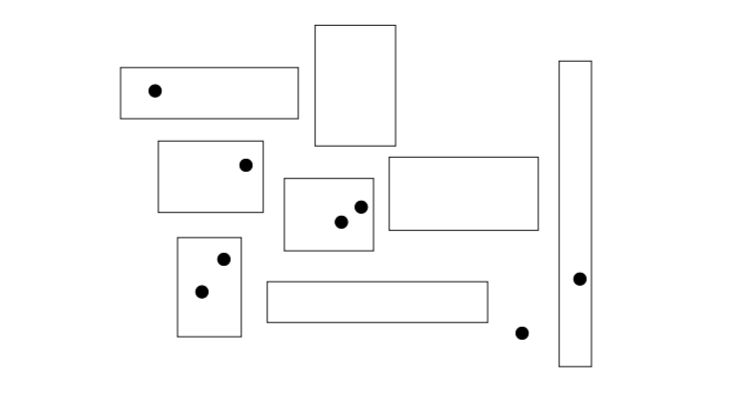
\includegraphics[width=4in]{points-rectangles.png}
\end{center}
\caption{Example of the general case of the problem.}

\end{figure}

\begin{enumerate}
\Q{10} First consider the special that when all rectangles of $R$ are assumed to intersect a given horizontal line $\ell$. Now design an $O(n\log(n))$-time algorithm for this special case.

\begin{figure}[h!]
\begin{center}
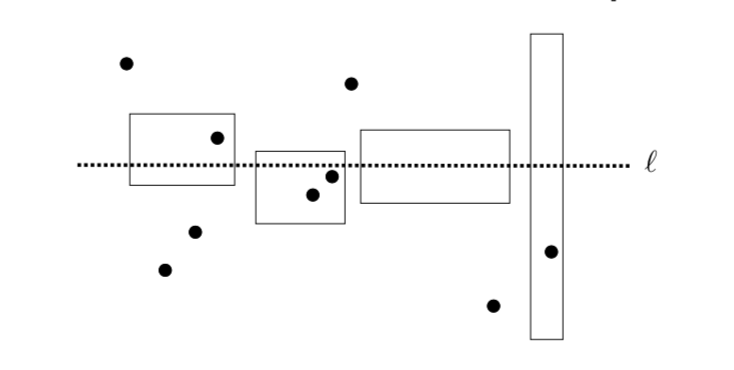
\includegraphics[width=4in]{points-rectangles-x-axis.png}
\end{center}
\caption{Example of the special case from Q3a.}
\end{figure}

Let $r \in R$, define $r.topLeft$ to be the coordinate of the top left point in $r$ and $r.botRight$ to be the 
coordinate of the bottom right point in $r$.\\
We first sort $R$ according to the x-coordinate of tge top left point of each rectangle. Then find the rectangle 
that contain $p \in P$ iteratively. For every $p \in P$, we use an algorithm that is similar to binary search 
to find the rectangle that contains $p$ or conclude that $p$ is not in any rectangle.

\begin{algorithm} [h]
    \caption{Find-Rec-l($P, R$)}

    \SetKwProg{Fn}{}{: }{end}
    \Fn{Rec-Cand($R, p$)} {
        \textbf{Iuput:} An array of rectangles sorted by the x-coordinate of the top left point 
        of each rectangle.\\
        \textbf{Output:} The index of the rectangle that may contain $p$.\\
        $lo = 1$\\
        $hi = \lvert R \rvert$\\
        \While {$lo \leq hi$} {
            $mid = \lfloor (lo + hi) / 2 \rfloor$\\
            \uIf {$R[mid].topLeft.x = P[i].x$} {
                \Return $mid$
                \textbf{Break}
            } \uElseIf {$R[mid].topLeft.x < P[i].x$} {
                $lo = mid + 1$\\
            } \Else {
                $hi = mid - 1$\\
            }
        }
        \Return $hi$
    }

    \SetKwProg{Fmain}{}{: }{end}
    \Fmain{Find-Rec-l($P, R$)} {
        \textbf{Ouput:} An array $A$ where $A[i]$ is a rectangle that contains $P[i]$ or $-$ if $P[i]$ is not in 
        any rectangle.\\
        sort($R$) such that $r_i.topLeft.x \leq r_j.topLeft.x$ for all $i < j, r_i, r_j \in R$\\
        \For {$i = 1 \cdots n_2$} {
            $j = Rec$-$Cand(R, P[i])$\\
            \eIf {$j = 0$ \textbf{or \\ not} 
            ($R[j].topLeft.x \leq P[i].x \leq R[j].botRight.x$ \textbf{and}
            $R[j].topLeft.y \leq P[i].y \leq R[j].botRight.y$)} {
                $A[i] = -$\\
            } {
                $A[i] = R[j]$\\
            } 
        }
        \Return $A$
    }
\end{algorithm}
\textbf{proof of correctness:} We prove that Rec-Cand($R, p$) always terminates and returns the index of  
a rectangle that we only need to compare. \\
The while loop in Rec-Cand($R, p$) always by the properties of binary search.\\
Since all rectangles intersect with a horizontal line $\ell$. Then there can't exist a rectangle $r$ such that 
$r'.topLeft.x \leq r.topLeft.x \leq r'.botRight.x$, $r'.topLeft.y \leq r.botRight.y$ or 
$r'.botRight.y \geq r.topLeft.y$ for some $r' \in R$. So if $R[i].topLeft.x \leq p.x \leq R[i + 1].topLeft.x$ 
for some point $p$, $p$ is either in $R[i]$ which has the largest top left x-coordinate that is smaller than 
$P.[i].x$ or not in any rectangle.\\
If $P[i].x = R[j].topLeft.x$ for some $1 \leq j \leq n$. By the proof above, we only have to check 
whether $P[i]$ is in $R[j]$.\\
If $P[i].x \neq R[j].topLeft.x$ for all $1 \leq j \leq n$. Since we take the midpoint every iteration, 
$1 \leq hi \leq n$. We claim $R[hi]$ has the largest top left x-coordinate that is smaller than $P[i]$. If 
$P[i].x$ is greater than all rectangle's top left x-coordinate, $lo$ would be $n + 1$ evetually and $hi$ is 
always $n$. Hence the statement holds. So we can assume $P[i].x$ is smaller than some x-coordinate in $R$. 
Then at some point, $hi$ is updated to $mid - 1$ where the element in the new value of $hi$ has a smaller 
x-coordinate since $p[i].x$ is not in $R$ but the element in $mid$ has a greater x-coordinate. Only $lo$ 
is updated after that points since $mid \leq hi$ and $R[hi].topLeft.x < P[i].x$. Hence the claim holds.
Bt the previous proof we only need to check $R[hi]$.\\
\textbf{Runtime analysis:} Rec-Cand($R, p$) takes $O(\log n_1)$ time. Hence Find-Rec-l($P, R$) has runtime 
$O(n_1 \log n_1) + n_2 O(\log n_1) = O(n \log n)$.

\newpage
\Q{12} Now give an $O(n\log^2(n))$-time algorithm (or better) for the general case of the problem. (Hint: use divide-and-conquer and use part (a) as a subroutine).\\
We start with a set $A$ that stores the answers and $A[i] = -$ for all $i$ at the beginning.
We put the x-coordinates of points and $\frac {r.topLeft.y + r.botRight.y} {2}$ into an array and sort them. Let 
$\ell$ be the median value of $B$. We determine whether a point is in the rectangles that intersect with $\ell$ by 
using the algorithm in part (a). Then divide the problem into two subproblems with size $\leq \frac n 2$.
At each recursion, we update the set that contains the answer.\\

\begin{algorithm} [h]
    \caption{Find-Rec($P, R$)}
    \SetKwProg{Fn}{}{: }{end}
    \Fn{Find-Rec-B($B$)} {
    \textbf{Input:}  $B = P \cup R$\\
    Let $A$ be a set that stores the answers. \\
    \If {$\lvert B \rvert = 0$ \textbf{or} ($\lvert B \rvert = 1$ \textbf{and} $B[1]$ is a point)} {
        \Return
    }
    $\ell = (r.topLeft.y + r.botRight.y) / 2$ if $B[n / 2]$ is a rectangle or $B[n / 2].y$ if $B[n / 2]$ 
    is a point.\\
    \For {$i = 1, \cdots, n$} {
        \If {$B[i]$ is a rectangle \textbf{and} $B[i].topLeft.y \leq \ell \leq B[i].botRight.y$} {
            $R_1 = R_1 \cup B[i]$\\
            $B = B \setminus B[i]$\\
        }
    }
    $A = \text{Find-Rec-l}(P, R_1)$\\
    Remove the points in $B$ that are in a rectangle in set $R_1$ and the points on $\ell$\\
    $n' = \lvert B \rvert$\\
    update $A$ based on $\text{Find-Rec}(B[1, \cdots, \lfloor n' / 2 \rfloor])$\\ 
    update $A$ based on $\text{Find-Rec}(B[\lfloor n' / 2 \rfloor + 1, \cdots, n'])$\\
    \Return $A$
    }

    \SetKwProg{Main}{}{: }{end}
    \Main{Find-Rec($P, R$)} {
        $B = P \cup R$\\
        Sort B according to $p.y$ or $(r.topLeft.y + r.botRight.y) / 2$ in ascending order.\\
        Find-Rec-B($B$)\\
    }
\end{algorithm}

\textbf{Proof correctness:} We compare all the points with every rectangle intersects with $\ell$. If a point 
is in one of the rectangle intersects with $\ell$, we can dorp this point since rectangles do not overlap. In 
addition, we can also drop the rectangles on $\ell$ since we have already compared them with all points. If a 
point $p$'s y-coordinate is greater than $\ell$ and $(r.topLeft.y + r.botRight.y) / 2$ is smaller than $\ell$ 
for a rectangle, we have already compared them by calling Find-Rec-l from part (a). So the division does not 
lose any solution. 
Eventually, we will remove all the rectangle or leave with only one point in $B$. The algorithm always 
terminates. Hence it is correct.\\
\textbf{Runtime analysis:} 
$T(n) = O(n \log n) + T'(n)$ where $T'(n)$ is the runtime of Find-Rec-B.\\
Assume $n > 1$, we have at most $n$ points and rectangles if we don't remove any rectangles or points. Then 
$B$ is divided into two parts where each part has length at most $\frac n 2$.
$T'(n) \leq 2 T(n / 2) + O(n) + O(n \log n) = 2 T'(n / 2) + O(n \log n)$\\
So, 
\begin{align*}
    T'(n) & = 2 T'(n / 2) + O(n \log n)\\
    & \leq \sum_{i = 1}^{\log n} c_i \cdot i \frac n i \log(\frac n i) \text{\quad by the definition of big-O}\\
    & \leq c n \sum_{i = 1}^{\log n} \log(\frac n i) \quad c = max\{c_1, \cdots, c_{\log n}\}\\
    & = c n \sum_{i = 1}^{\log n} \log n - \log i\\
    & \leq c n \sum_{i = 1}^{\log n} \log n\\
    & = c n \log^2 n\\
    & = O(n \log^2 n)
\end{align*}
Therefore, $T(n) =  O(n \log n) + O(n \log^2 n) = O(n \log^2 n)$
\end{enumerate}

\newpage
\Q{15} Your friend has invited you to play a game which goes as follows. There are two sets of sticks: (i) $R$ that consists of $n$ red sticks; and $B$ that consists of $n$ blue sticks. Each stick has a height (you can assume they are distinct for simplicity). Each player pairs red and blue sticks (so creates $n$ pairs of stick, where each pair contains one red and one blue stick) and the winner is the one that minimizes the ``sum, across all pairs, the differences in heights. So suppose you have paired the sticks and in your $i$'th pair the height of red stick is $r_i$ and the height of the blue stick be $b_i$, then you incur $|r_i-b_i|$ penalty. Design an algorithm that runs in $O(n \log n)$ time (or better) that pairs the sticks with the minimum possible penalty. In other words, your algorithm minimizes the following sum across all possible pairings:

$$\Sigma_{i=1\ldots n} |r_i - b_i|$$

We sort two arrays and pair $R[i], B[i]$

\begin{algorithm} [h]
    \caption{PairSticks($R, B$)} {
        \textbf{Output:} $A$\\
        Sort $R$ by heights in ascending order.\\
        Sort $B$ by heights in ascending order.\\
        \For {$i = 1, \cdots, n$} {
            $A[i] = (R[i], B[i])$\\
        }
        \Return $A$
    }
\end{algorithm}

\textbf{Proof of correctness:} We claim that the algorithm above is optimal.\\
Let $A' = {(r_1, b_1), (r_2, b_2), \cdots, (r_n, b_n)}$ be the 
set that a random algorithm returns. There exists two pairs $(r_i, b_i)$ and $(r_j, b_j)$ such that $r_i \leq r_j$ 
and $b_j \leq b_i$. Let $a, c$ be the one with smaller height in the two pairs and $b, d$  be the one with greater 
height in the two pairs. We have $a \leq c \leq d \leq b$. If $a$ and $c$ do not have same color, we can swap 
$a$ and $c$ to get a even smaller penalty. If $a$ and $c$ have same color, then the penalty of the pairs $(a, d)$ 
and $(c, b)$ is $d - a + b - c = d - c + c - a + b - d + d - c = (b - d + d - c + c - a) + (d - c) = b - a + d - c$. 
$b - a + d - c$ is the penalty of $(a, b)$ and $(c, d)$.\\
Hence the algorithm above is optimal.
\textbf{Runtime analysis:} Sorting $R$ and $B$ take $2O(n \log n) = O(n \log n)$ time. Pairing each element takes 
$O(n)$ time. hence the overall runtime is $O(n \log n)$. 

\end{enumerate}

\end{document}

